\section{Datapath Optimization} \label{sec:dtptopti}
According to \cite{chen_eyeriss_2017}, the data-movement can often be more energy-consuming than actual computation. Smart memory management is then required to implement a \acrshort{cnn} on low power device such as \acrshort{fpga}.
%
%
\subsection{Systolic Arrays}
%
%
Systolic arrays were implemented on the first \acrshort{fpga}-based accelerators. A static systolic array is a static array of \acrshort{pe} doing a part of the computation and communicating with its neighbors. An illustration of its principle can be found on figure \ref{fig:sytar}. The configuration can only support convolution with a kernel size $K_*$ lower than a bound, such that $K_* \leq K_m$. The systolic array allows spatial data reutilisation between rows and columns and temporal data reutilisation.\newline \newline
\begin{figure}
    \centering
    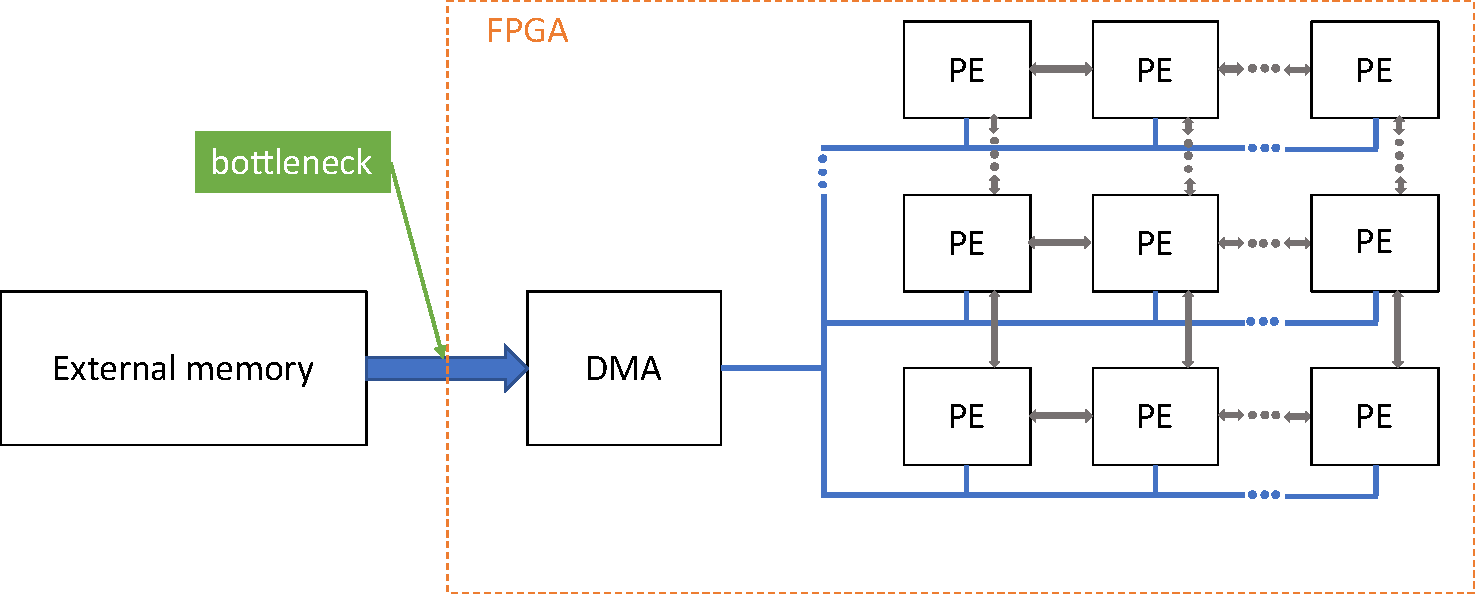
\includegraphics[width=\textwidth]{systArray.pdf}
    \caption{Static Systolic Arrays}
    \label{fig:sytar}
\end{figure}
However, Systolic Arrays has also issues. First, when the kernel size is much lesser than the maximal kernel size ($K_* << K_m$), there is an underutilization of the resources. For example, \cite{gokhale_240_2014} notes that for a $3 \times 3$ kernel, only $9\%$ of the \acrfull{dsp} blocks are used. Second,  data caching is not implemented. It means that it has always to fetch input from the external memory. Memory becomes the bottleneck and the performance is bounded by the device memory bandwidth.
%
%
\subsection{Data-flow \acrshort{moc} for \acrshort{cnn}s}
%
%
Data-flow \acrfull{moc} can be used to accelerate \acrshort{cnn}s on \acrshort{fpga}. This approach is motivated because the feed-forward aspect of the inference stage of the \acrshort{cnn} is purely data driven.
Data-flow \acrfull{moc} were firstly investigated by \cite{lin_li_low_2016}.  We describe the \acrshort{cnn} as a network where:
\begin{itemize}
    \item \textbf{nodes} are processing unit called an \textit{actor}. Each actor follows a data-driven exectution where the execution is triggered by the availability of input, which is the case for a \acrshort{cnn}.
    \item \textbf{edges} are communication \acrshort{fifo} channels. Actors exchange data called \textit{tokens} through those \acrshort{fifo} channels.
\end{itemize}
A represention of such network can be found in figure \ref{fig:moc}. \newline \newline
The \acrshort{cnn} can be therefore modeled as a topology matrix and we only have to explore those matrix components (instead of tiling and unrolling parameters of section \ref{subsec:loopopti}) to minimize latency or energy consumption. Those parameters are then used to derive \acrshort{pe} and buffer configuration. However, as pointed by \cite{abdelouahab_tactics_2017}, the direct hardware mapping of \acrshort{cnn} network means that all the computations must be unrolled, we are then bounded by the hardware resources and the size of the \acrshort{cnn}, preventing implementing this approach for deep models.
\begin{figure}
    \centering
    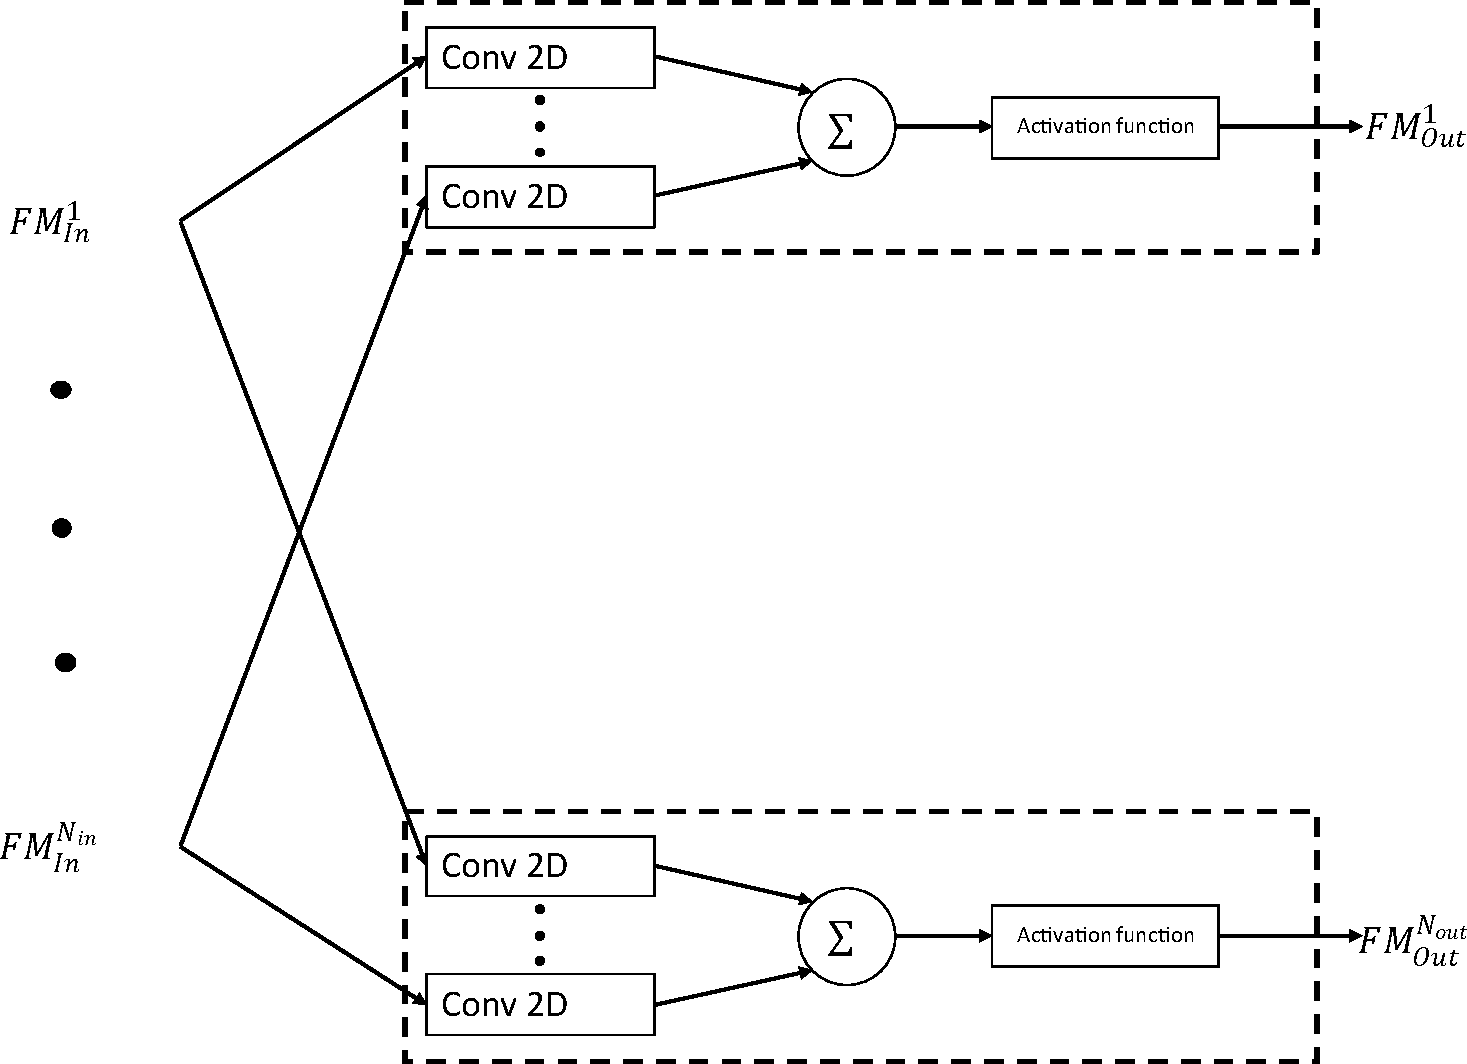
\includegraphics[width=0.8\textwidth]{Moc.pdf}
    \caption{Graph represenation of a convolution layer}
    \label{fig:moc}
\end{figure}
%
%
\subsection{Loop Optimization} \label{subsec:loopopti}
%
%
Loop optimizations techniques were already described at section \ref{sec:loopopti}. Unrolling parameters, tiling parameters and loop ordering are up to the programmer to set. We are going to review different works who have studied the design space exploration of such parameters to design the most efficient accelerator that would be feasible on the target. \newline \newline
%
The work of \cite{zhang_optimizing_2015} proposes an analytical solution using the roofline model \cite{williams_roofline_2009} to identify the CNN design with best performance and lowest \acrshort{fpga} resource requirement. They have chosen a loop unrolling of ($T_{if} \times T_{of}$) to avoid complex connection topologies for all arrays. It allows a spatial reutilisation of pixels for $T_{of}$ unrolls, and the temporal reutilisation of weight for ($T_{ox} \times T_{oy}$). We can observe their accelerator structure on figure \ref{lst:accelerator}. However, the disadvantage of this method is the need of a large local memory to store the partial sums ($T_{of} \times T_{ox} \times T_{oy}$).
%
\begin{figure}
    \centering
    \begin{lstlisting}[language=Java]
// Load weights
// Load input FM
% on-chip data computation
for(kx=0; kx<Nkx; kx+=1){
    for(ky=0; ky<Nky; ky+=1){
        for(tix=0; tix<min(ix+Tix, Nix); tix+=1){
            for(tiy=0; tiy<min(iy+Tiy, Niy); tiy+=1){
                for(tof=0; tof<min(of+Tof, Nof); tof+=1){
                #pragma HLS UNROLL
                    for(tif=0; tif<min(if+Tif, Nif); tif+=1){
                    #pragma HLS UNROLL
                    L : output_fm[tof][tix][tiy] +=
                    weights[tof][tif][kx][ky]*
                    input_fm[tif][S*tix+kx][S*tiy+ky];
                    }
                }
            }
        }
    }
}
// Load input FM
    \end{lstlisting}
    \caption{Architecture loop ordering \cite{zhang_optimizing_2015}}
    \label{lst:accelerator}
\end{figure} \newline
%
Once the loop ordering and unrolling parameters have been set, the roofline methode can be used to find the optimal tiling parameters. This design exploration method uses two limits to find the best trade-off between memory bandwith and computational speed:
\begin{enumerate}
    \item \textbf{Computational roof}: $= \frac{\text{\# of operations}}{\# of execution cycles}$.
    \item \textbf{CTC ratio}: $= \frac{\text{\# of operations}}{\# of external data access}$
\end{enumerate}
As an implementation can either be computation-bounded or memory-bounded, we can compute the attainable performance as equation \ref{eq:atperf}.
\begin{equation}
Att \ perf = min(Computational \ roof; CTC \ ratio \times bandwith)
\label{eq:atperf}
\end{equation}
The roofline method is shown of figure \ref{fig:roofmeth}. In this figure, the implementation C and D achieves the highest possible performance on the \acrshort{fpga}. However, the implementation C is prefered because it requires least bandwith.
%
\begin{figure}
    \centering
    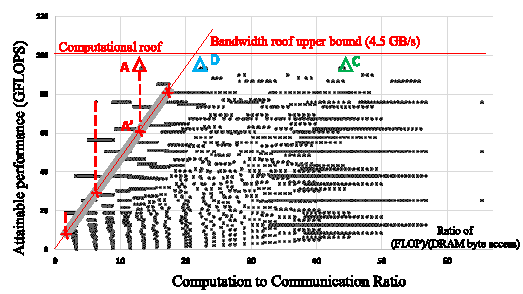
\includegraphics[width=\textwidth]{roofmethod.pdf}
    \caption{Design space of platform-supported designs  \cite{zhang_optimizing_2015}}
    \label{fig:roofmeth}
\end{figure} \newline \newline
%
\cite{motamedi_placid_2017} ises tiling and on-chip memory, and propose Fat Convolution Engines which are characterized by two extra parameters: $\omega$ the bus with and $P$ the number of ports. Moreover, it selects the best data access optimization with the higher performance based on the hyper-parameters.
%
A different approach has been studied by \cite{ma_optimizing_2018}. It proposes a design space exploration regarding to the various design objectives. They have proposed two flowcharts on figure \ref{fig:flowchart} in order to
\begin{itemize}
    \item \textbf{Latency}: $P_*$ should be common factors of  $T_*$ for all convolution layers to fully utilize \acrshort{pe}s, and $T_*$ to be the common factors of  $N_*$ to make full use of external memory transactions.
    \item \textbf{Partial sum storage}: to minimize the concurrent storage of partial sums in local memory and allowing to keep them into the PE, we should prior the computation of an output pixel in order to evacuate it to the external memory.
    \item \textbf{On-chip memory access}: on-chip memory access can be minimized by reusing at most pixels or weights in the \acrshort{pe}s.
    \item \textbf{External memory access}: to minimize external access, a sufficient buffer size should be assigned to pixels and weights.
\end{itemize}
%
\begin{figure}
\centering
    \begin{subfigure}{.45\textwidth}
    \centering
    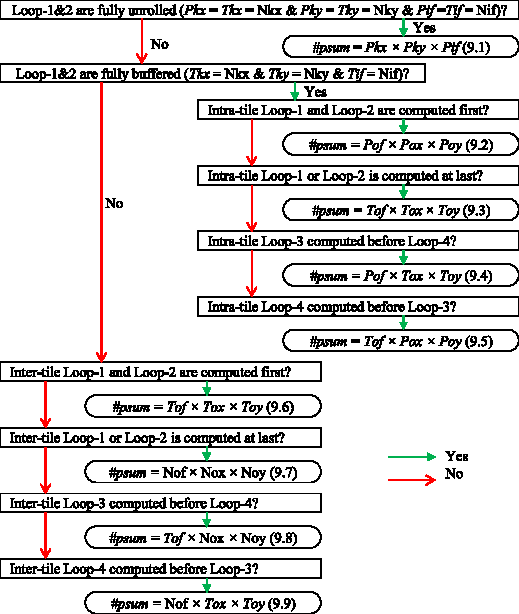
\includegraphics[width=\linewidth]{fwch1.pdf}
    \caption{ }
    \end{subfigure}
    \begin{subfigure}{.45\textwidth}
    \centering
    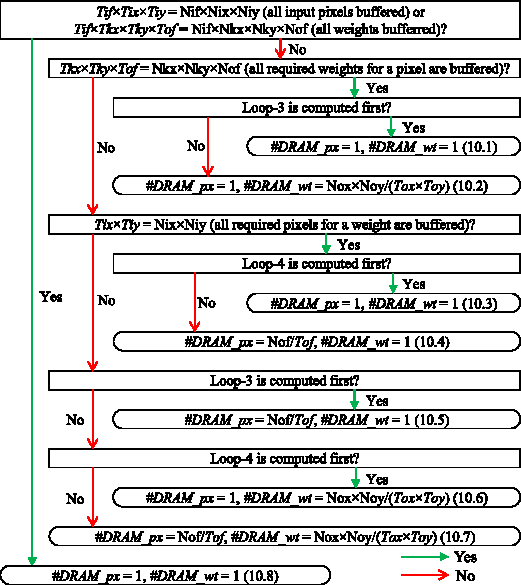
\includegraphics[width=\linewidth]{fwch2.pdf}
    \caption{ }
    \end{subfigure}
    \caption{Design space exploration of: (a) total number of partial sums that need to be stored in memory; (b) the number of external memory accesses \cite{ma_optimizing_2018}}
    \label{fig:flowchart}
\end{figure}
